\chapter{DeepInf: Social influence prediction}


\section{Introduction}
\paragraph{} Deepinf focus on the prediction of user-level social influence. It aims to \textbf{predict the action status of a user given the action}.
It is a deep learning based framework to represent both influence dynamics and network structures into a latent space and 
tries to minimize the negative likelihood that was defined in the section 1.


\section{Model framework}
\subsection{Sampling Near Neighbour}

\paragraph{} Give a user $v$, a r-ego network $\mathcal{G}_v^r$ is extracted using breadth-first search (BFS) starting from 
user $v$. However, $\mathcal{G}_v^r$ may have different size due to the small world property in the social network. Since most
deep learning models expects fixed size data, the graph $\mathcal{G}_v^r$ can be sampled to fixed size.
\paragraph{} For sampling a fixed size graph \textbf{random walk the restart} (RWR) was used. RWR algorithm is defined as
following steps.

\begin{itemize}
    \item Start random walks from either the ego user $v$ or one of her active neighbors randomly.
    \item The random walk iteratively travels to its neighborhood with the probability that is 
    proportional to the weight of each edge.
    \item At each step, the walk is assigned a probability to return to the starting node, that is, 
    either the ego user $v$ or one of $v$’s active neighbors.
    \item Run the algorithm until a fixed number of vertices denoted by $\hat{\Gamma_v^r}$ with $\hat{|\Gamma_v^r|}$=n. 
\end{itemize}

\paragraph{} After running this algorithm, a sub-graph $\hat{\mathcal{G}_v^r}$ and denote $\hat{S}_v^t$=
\{ $s_u^t :u \in \hat{\Gamma_v^r}$ \} be the action statuses of $v$'s sampled neighbours. Therefore we re-define the optimization
objective in section 1 as:

\begin{equation}
    \mathcal{L}(\theta) = -\sum_{i=1}^N \log(P_{\theta}(s_{v_i}^{t_i+\Delta t}|\hat{\mathcal{G}_{v_i}^{t}},s_{v_i}^{t_i}))
\end{equation}


\subsection{Neural Network}
\paragraph{} With the retreived $\hat{\mathcal{G}_{v_i}^{t}}$ and $\hat{S}_v^t$ for each user, an effective
neural network model to incorporate both the structural properties in $\hat{\mathcal{G}_{v_i}^{t}}$ and action statuses in 
$\hat{S}_v^t$.

\begin{figure}
    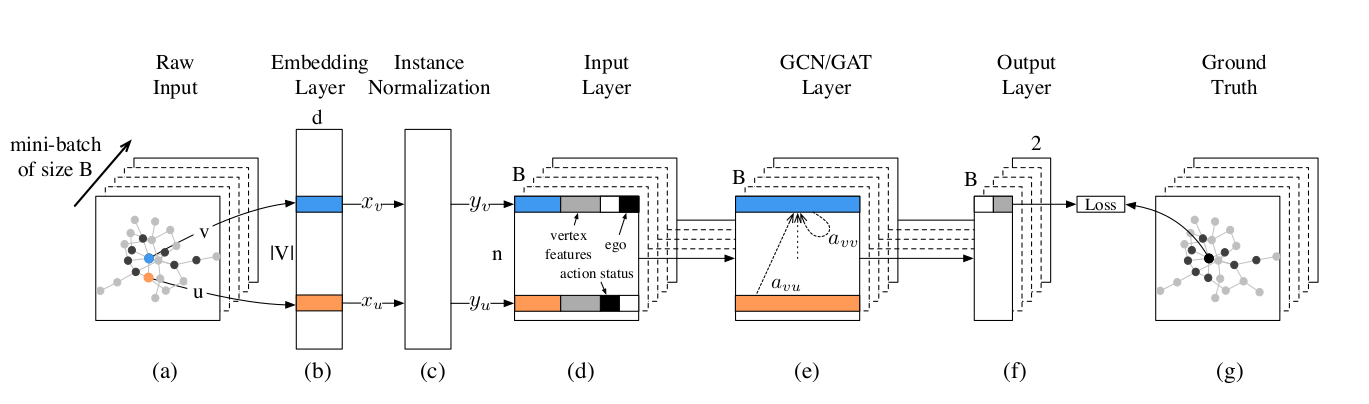
\includegraphics[width=12cm,height=4cm]{tex/img/framework.png}
\end{figure}

\paragraph{} Deepinf neural network model consist of network embedding layer, instance normalization layer, input layer
and GCN layer as described in the above diagram.


\subsubsection{Embedded layer}

\paragraph{} Network embedding technique encode network structural properties into low dimensional matrix $\mathbf{X} \in
\mathcal{R}^{\mathcal{D} \times |V|}$. Deepinf uses Deepwalk algorithm for mapping each users into $\mathcal{R}^{\mathcal{D}}$
space.


\subsubsection{Instance Normalization}

\paragraph{} Instance normalization can remove instance-specific mean and variance, which encourages the downstream model 
to focus on users’ relative positions in latent embedding space rather than their absolute positions. It also prevents 
overfitting.

\paragraph{} Let $x_u$ be the low dimension representation for the user $u \in \hat{\Gamma_v^r}$, the instance normalized
vector $y_u$ is obtained by

\begin{equation}
    y_{ud} = \frac{x_{ud}-\mu_{ud}}{\sqrt{\sigma_d^2+\epsilon}}
\end{equation}

for each embedding dimension d = 1...$\mathcal{D}$, where 
\begin{equation}
    \mu_d = \frac{1}{n}\sum_{u \in \hat{\Gamma_v^r}}x_{ud},\ \sigma_d^2 = \frac{1}{n}\sum_{u \in \hat{\Gamma_v^r}}(x_{ud}-\mu_{ud})^2
\end{equation}


\subsubsection{Input Layer}

\paragraph{} Input later constructs feature vector for each user. Along with the output from the instance Normalization,
input layer adds two binary variable. The first variabe indicates user's action status and second variable indicates whether
the user is the ego user.

\subsubsection{GCN}

\paragraph{} Graph Convolutional Network (GCN) was discussed in detail in the previous chapter. Given the node features 
matrix $\mathcal{H} \in \mathcal{R}^{n \times F}$, for $n$ nodes in the sub-graph, GCN tries to extract neighbourhood 
information for all the nodes in the subgraph and projects into lower dimensional space.

\subsubsection{Output layer and loss function}

\paragraph{} The output layer produces a two dimension representation for each users and comparing the representation for
the ego user with the ground truth value the negative log-likelihood (Eq 3.1) is minimized.

\section{Experimentation}

\subsection{Dataset}

\subsubsection{Digg}
\begin{itemize}
    \item Digg is a \textbf{news aggregator which allows people to vote web content, a.k.a, story, up or down}.
    \item The dataset contains data about stories promoted to Digg’s front page over a period of a month in 2009.
    \item For each story, it contains the list of all Digg users who have voted for the story up to the 
    time of data collection and the time stamp of each vote.
\end{itemize}

\subsubsection{Data preparation}
\begin{itemize}
    \item As dataset is imbalanced (negative instances are more than positive instances), the data is sampled to achieve a balanced distribution.
    \item Each subgraph for the user $v$, has fixed neighbors (50).
\end{itemize}

\subsection{Evaluation metrics}
\paragraph{} The model was trained for 1000 epochs and prediction performance like AUC, Precision, Recall, F1-Score were calculated.
\begin{center}
    \begin{tabular}{ |c|c|c|c|c|c| } 
     \hline
     \textbf{Data} & \textbf{Model} & \textbf{AUC} & \textbf{Precision} & \textbf{Recall} & \textbf{F1} \\ 
     \hline
     Digg & DeepInf+GCN (Our's) & 0.82 & 0.58 & 0.634 & 0.604\\ 
     Digg & DeepInf+GCN (Author's) & 0.84 & 0.587 & 0.676 & 0.6288\\ 
     \hline
    \end{tabular}
    \end{center}
\subsubsection{Precision Recall plots}
\begin{figure}[h]
    \centering
    \begin{subfigure}[b]{0.5\textwidth}
                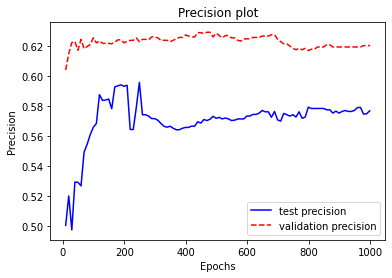
\includegraphics[width=\textwidth,height=4cm]{tex/img/precision_plot.png}
                \caption{Precision plot}
        \end{subfigure}%
        \hfill
    \begin{subfigure}[b]{0.5\textwidth}
                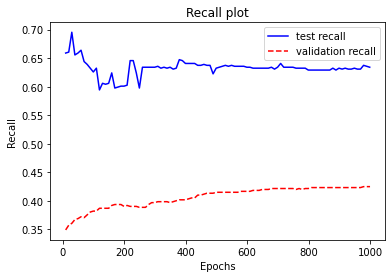
\includegraphics[width=\textwidth,height=4cm]{tex/img/recall_plot.png}
                \caption{Recall plot}
       \end{subfigure}%
    \end{figure}
\subsubsection{Loss f1-score plots}
\begin{figure}[h]
    \centering
    \begin{subfigure}[b]{0.5\textwidth}
                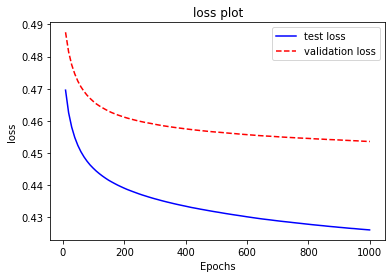
\includegraphics[width=\textwidth]{tex/img/loss_plot.png}
                \caption{Loss plot}
        \end{subfigure}%
        \hfill
    \begin{subfigure}[b]{0.5\textwidth}
                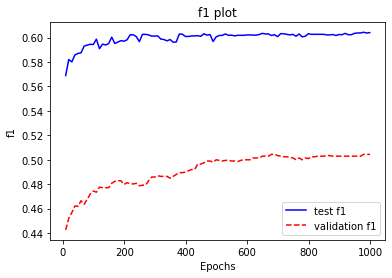
\includegraphics[width=\textwidth]{tex/img/f1_plot.png}
                \caption{F1-score plot}
       \end{subfigure}%
    \end{figure}


